\section{问题四的波动电价模型}

\subsection{因果价格预测}

实时电价沿用问题二的三个因果基预测器和动态权重，正式回测期 MAE、RMSE 和 WAPE
分别为 0.0524 元/kWh、0.0705 元/kWh 和 $6.9211\%$。日前优化使用
$\widehat p_{d,t}$，日内发布时刻以后再根据已观察价格偏差修正未来预测；最终计划费、
调整费和紧急购电费全部按真实 $p_{d,t}$ 重算。

问题 4-2 的费用为
\begin{equation}
C_{4-2}=\sum_{d,t}p_{d,t}x_{d,t}
+5\sum_{d,t}p_{d,t}u_{d,t}.
\end{equation}
问题 4-3 沿用式~(\ref{eq:adjust})，只是每个时段采用相应的真实价格结算。为度量价格信息价值，另在不改变负载与光伏预测边界的前提下，把完整当日价格提供给优化器，形成完美价格信息对照。

\subsection{计算结果}

波动电价下，问题 4-2 的计划费为 $1398.08$ 万元，紧急购电费为
$183.30$ 万元，总费用为 $1581.38$ 万元；问题 4-3 的初始计划费、调整费和紧急费分别为
$1423.30$ 万元、$96.74$ 万元和 $26.78$ 万元，总费用为 $1546.83$ 万元。
滚动光伏预报使同一价格制度下总费用下降 $34.55$ 万元，并将紧急购电量从
$27.84$ 万 $\mathrm{kWh}$ 降至 $5.37$ 万 $\mathrm{kWh}$。

完美日内价格信息下问题 4-2 的总费用为 $1576.25$ 万元，比因果价格预测少
$5.13$ 万元。该差额约占主方案费用的 $0.32\%$，说明现有价格预测已捕捉主要日内结构，但极端价格区间仍有改进空间。

\begin{figure}[H]
  \centering
  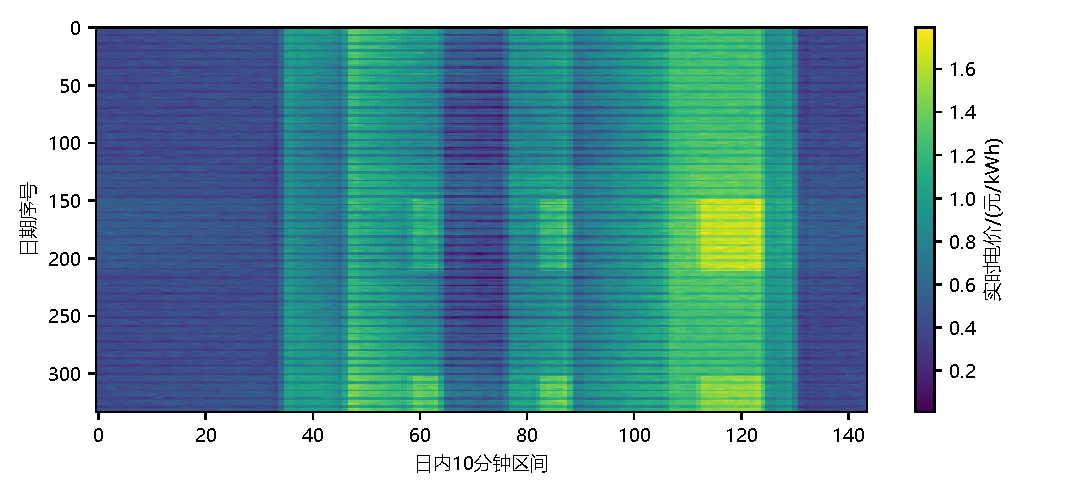
\includegraphics[width=0.9\textwidth]{../figures/p4_price_heatmap.pdf}
  \caption{提交期实时电价的日期--区间分布}
  \label{fig:p4price}
\end{figure}

\begin{figure}[H]
  \centering
  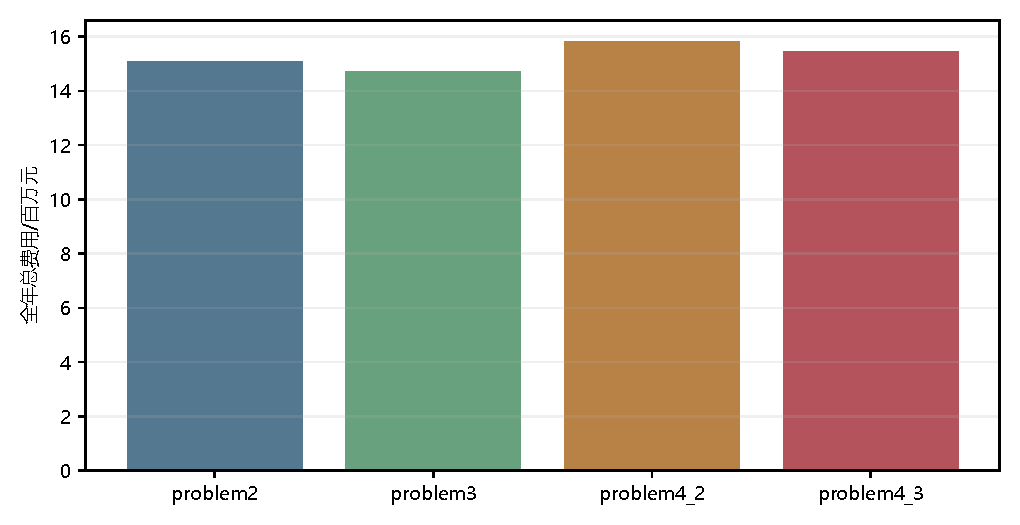
\includegraphics[width=0.82\textwidth]{../figures/scenario_cost_comparison.pdf}
  \caption{固定与波动电价下四种主场景总费用}
  \label{fig:costcompare}
\end{figure}

固定价格和波动价格的绝对费用不宜直接用于评价策略优劣，因为结算价格制度不同。更有意义的比较是在同一价格制度下观察滚动预报相对日前策略的成本下降和紧急购电减少。
